\documentclass[11pt,a4paper]{article}
\usepackage[utf8]{inputenc}
\usepackage[T1]{fontenc}
\usepackage[scaled=0.92]{helvet}
\renewcommand{\familydefault}{\sfdefault}
\usepackage[a4paper,margin=2.2cm,headheight=14pt]{geometry}
\usepackage{microtype}
\usepackage[table]{xcolor}
\usepackage{booktabs,tabularx,longtable,array,enumitem,parskip,float,caption}
\usepackage{fancyhdr,titlesec}
\usepackage[most]{tcolorbox}
\usepackage{tikz}
\usetikzlibrary{arrows.meta,positioning}
\usepackage{listings}
\usepackage{amssymb}
\usepackage[hidelinks]{hyperref}

\definecolor{navy}{HTML}{1F2A44}
\definecolor{ermgreen}{HTML}{2E7D32}
\definecolor{ermamber}{HTML}{F9A825}
\definecolor{ermred}{HTML}{C62828}
\definecolor{tintgreen}{HTML}{C8E6C9}
\definecolor{tintamber}{HTML}{FFF3C4}
\definecolor{tintred}{HTML}{F8CACA}
\definecolor{softgrey}{HTML}{F2F4F7}

\titleformat{\section}{\Large\bfseries\color{navy}}{\thesection}{0.8em}{}[{\color{navy}\titlerule[0.8pt]}]
\titleformat{\subsection}{\large\bfseries\color{navy}}{\thesubsection}{0.6em}{}
\titlespacing*{\section}{0pt}{1.3em}{0.7em}
\pagestyle{fancy}\fancyhf{}
\fancyhead[L]{\small\color{gray}Panduan Perakitan Dashboard Power BI --- ERM Framework ASB (fiktif)}
\fancyfoot[L]{\small\color{gray}Bank fiktif \textbullet{} data sintetis}
\fancyfoot[R]{\small\color{gray}Halaman \thepage}
\renewcommand{\headrulewidth}{0.4pt}
\renewcommand{\contentsname}{Daftar Isi}
\renewcommand{\tablename}{Tabel}
\setlist[itemize]{topsep=2pt,itemsep=2pt}
\setlist[enumerate]{topsep=2pt,itemsep=3pt}
\renewcommand{\arraystretch}{1.22}
\newtcolorbox{tipbox}[1][Tips]{colback=tintgreen!45,colframe=ermgreen,fonttitle=\bfseries,title={#1},boxrule=0.6pt,arc=2pt,left=6pt,right=6pt}
\newtcolorbox{warnbox}[1][Perhatian]{colback=tintamber!60,colframe=ermamber!90!black,coltitle=black,fonttitle=\bfseries,title={#1},boxrule=0.6pt,arc=2pt,left=6pt,right=6pt}
\newtcolorbox{infobox}[1][Catatan]{colback=softgrey,colframe=navy,fonttitle=\bfseries,title={#1},boxrule=0.6pt,arc=2pt,left=6pt,right=6pt}
\newtcolorbox{stepbox}[1]{colback=white,colframe=navy!70,fonttitle=\bfseries,title={#1},boxrule=0.5pt,arc=2pt,left=6pt,right=6pt}
\lstset{basicstyle=\ttfamily\small,backgroundcolor=\color{softgrey},frame=single,rulecolor=\color{gray!40},
  columns=fullflexible,keepspaces=true,breaklines=true,xleftmargin=4pt,xrightmargin=4pt,aboveskip=5pt,belowskip=5pt}
\newcommand{\file}[1]{\texttt{\small #1}}
\newcommand{\ui}[1]{\textbf{\textit{#1}}}
\begin{document}
\sloppy

\begin{center}
{\color{navy}\rule{\linewidth}{1.6pt}}\\[0.8em]
{\LARGE\bfseries\color{navy} Panduan Perakitan Dashboard Power BI}\\[0.4em]
{\large ERM Framework --- PT Amanah Syariah Bank (fiktif)}\\[0.4em]
{\small Lanjutan setelah 13 file CSV berhasil diimpor \textbullet{} posisi data September 2026}\\[0.6em]
{\color{navy}\rule{\linewidth}{0.8pt}}
\end{center}

\begin{infobox}[Di mana posisi Anda sekarang]
13 tabel sudah masuk ke Power BI Desktop. Langkah berikutnya: (1) merapikan tipe data, (2) membuat 21 relasi, (3) memasang measure DAX, (4) menyusun 6 halaman visual, (5) verifikasi angka. Ikuti berurutan; bagian \ref{sec:relasi} adalah yang sedang Anda kerjakan.
\end{infobox}

\tableofcontents
\newpage

\section{Ringkasan model: 5 dimensi, 8 fakta}

Model ini berbentuk \emph{star schema}. Tabel \file{dim\_} berisi daftar induk (tanggal, risiko, KRI, skenario, unit kerja). Tabel \file{fact\_} berisi angka. Arah filter selalu \textbf{dari dim ke fact}.

\begin{center}
\begin{tabularx}{\linewidth}{>{\ttfamily\small}p{4.3cm}r>{\raggedright\arraybackslash}X}
\toprule
\textrm{\textbf{Tabel}} & \textbf{Baris} & \textbf{Isi} \\
\midrule
dim\_date & 12 & Bulan Okt-2025 s.d. Sep-2026 \\
dim\_risk & 11 & 10 jenis risiko + Capital Overlay \\
dim\_kri & 43 & 42 KRI + CAP01 beserta batas c1--c4 \\
dim\_scenario & 4 & Actual, Baseline, Adverse, Severe \\
dim\_business\_unit & 16 & Pemilik KRI/tindakan \\
\midrule
fact\_kri\_monthly & 516 & 43 indikator $\times$ 12 bulan (nilai, skor, trend) \\
fact\_risk\_score & 150 & 10 risiko $\times$ (12 bulan Actual + 3 skenario) \\
fact\_enterprise & 15 & 12 bulan Actual + 3 skenario \\
fact\_stress & 129 & 43 indikator $\times$ 3 skenario \\
fact\_capital & 3 & KPMM per skenario \\
fact\_actions & 10 & Tracker tindakan \\
fact\_emerging & 3 & Register risiko baru \\
fact\_interdependency & 11 & Jalur antar-risiko (tabel berdiri sendiri) \\
\bottomrule
\end{tabularx}
\end{center}

\section{Langkah 1 --- Rapikan tipe data sebelum membuat relasi}\label{sec:tipe}

Relasi sering gagal hanya karena tipe kolom kunci berbeda (misalnya satu \emph{Whole Number}, satunya \emph{Text}). Rapikan dulu.

\begin{stepbox}{1.1 Periksa kolom kunci}
Buka \ui{Table view} (ikon tabel di kiri). Untuk setiap tabel, klik kolom yang namanya berakhiran \file{\_key}, lalu di ribbon \ui{Column tools} $\rightarrow$ \ui{Data type} pilih \ui{Whole number}. Kolom yang harus bertipe Whole number:
\begin{itemize}
\item \file{date\_key}, \file{risk\_key}, \file{kri\_key}, \file{scenario\_key}, \file{bu\_key}
\item \file{fact\_emerging[primary\_risk\_key]}, \file{fact\_interdependency[source\_risk\_key]}, \file{fact\_interdependency[target\_risk\_key]}
\end{itemize}
\end{stepbox}

\begin{stepbox}{1.2 Tipe lain yang perlu benar}
\begin{itemize}
\item \file{dim\_date[month\_start]} dan \file{[month\_end]}: \ui{Date}
\item \file{fact\_actions[due\_date]}: \ui{Date}
\item \file{fact\_kri\_monthly[early\_warning\_flag]}, \file{dim\_date[is\_reporting\_date]}, \file{fact\_actions[is\_overdue]}: \ui{True/False}
\item Kolom angka seperti \file{value}, \file{utilization}, \file{final\_score}, \file{kpmm}: \ui{Decimal number}
\end{itemize}
\end{stepbox}

\begin{warnbox}[Jika angka desimal terbaca salah]
Jika \file{final\_score} 2.65 terbaca 265, impor memakai locale Indonesia. Perbaiki di \ui{Transform data} $\rightarrow$ pilih tabel $\rightarrow$ langkah \ui{Changed Type} $\rightarrow$ ganti dengan \ui{Using Locale} $\rightarrow$ \ui{English (United States)}, lalu \ui{Close \& Apply}.
\end{warnbox}

\begin{stepbox}{1.3 Urutan tampilan (sekali saja, hasilnya rapi)}
\begin{itemize}
\item \file{dim\_date[month\_label]} $\rightarrow$ \ui{Column tools} $\rightarrow$ \ui{Sort by column} $\rightarrow$ \file{month\_index}
\item \file{dim\_risk[risk\_type]} $\rightarrow$ \ui{Sort by column} $\rightarrow$ \file{sort\_order}
\item \file{dim\_scenario[scenario]} $\rightarrow$ \ui{Sort by column} $\rightarrow$ \file{sort\_order}
\end{itemize}
\end{stepbox}

\begin{warnbox}[Jangan pakai ``Mark as date table'']
\file{dim\_date} hanya berisi 12 baris bulanan, bukan tanggal harian berurutan. Power BI menolak tabel seperti ini sebagai \emph{date table}, dan fungsi \emph{time intelligence} (DATEADD, SAMEPERIODLASTYEAR) tidak akan bekerja. Model ini memang tidak memakainya: perbandingan antar bulan memakai kolom \file{month\_index}. Lewati saja menu tersebut.
\end{warnbox}

\section{Langkah 2 --- Membuat 21 relasi}\label{sec:relasi}

\subsection{Aturan yang berlaku untuk semua relasi}

\begin{center}
\begin{tabularx}{\linewidth}{>{\bfseries}p{4.2cm}X}
\toprule
Pengaturan & Nilai \\
\midrule
Cardinality & \ui{Many to one (*:1)} bila Anda menarik dari fact ke dim, atau \ui{One to many (1:*)} bila menarik dari dim ke fact. Intinya: sisi \textbf{dim} = 1, sisi \textbf{fact} = banyak. \\
Cross filter direction & \ui{Single} (dim memfilter fact, tidak sebaliknya) \\
Make this relationship active & \ui{Dicentang} untuk seluruh 21 relasi \\
Assume referential integrity & Biarkan \textbf{tidak dicentang} \\
\bottomrule
\end{tabularx}
\end{center}

\subsection{Cara tercepat: lewat menu Manage relationships}

\begin{stepbox}{Langkah per relasi}
\begin{enumerate}
\item Buka \ui{Model view} (ikon paling bawah di kiri).
\item Klik ribbon \ui{Home} $\rightarrow$ \ui{Manage relationships} $\rightarrow$ \ui{New}.
\item Tabel atas: pilih tabel \file{dim\_...}, lalu klik judul kolom kuncinya (kolom ikut tersorot).
\item Tabel bawah: pilih tabel \file{fact\_...}, lalu klik judul kolom kuncinya.
\item Pastikan \ui{Cardinality} = \ui{One to many (1:*)} dan \ui{Cross filter direction} = \ui{Single}.
\item Klik \ui{OK}. Ulangi untuk semua baris pada tabel berikut.
\end{enumerate}
\end{stepbox}

\begin{longtable}{r>{\ttfamily\small}p{6.0cm}>{\ttfamily\small}p{6.6cm}}
\toprule
\textbf{No} & \textrm{\textbf{Dari (sisi 1)}} & \textrm{\textbf{Ke (sisi banyak)}} \\
\midrule
\endhead
1 & dim\_date[date\_key] & fact\_kri\_monthly[date\_key] \\
2 & dim\_kri[kri\_key] & fact\_kri\_monthly[kri\_key] \\
3 & dim\_risk[risk\_key] & fact\_kri\_monthly[risk\_key] \\
4 & dim\_date[date\_key] & fact\_risk\_score[date\_key] \\
5 & dim\_scenario[scenario\_key] & fact\_risk\_score[scenario\_key] \\
6 & dim\_risk[risk\_key] & fact\_risk\_score[risk\_key] \\
7 & dim\_date[date\_key] & fact\_enterprise[date\_key] \\
8 & dim\_scenario[scenario\_key] & fact\_enterprise[scenario\_key] \\
9 & dim\_date[date\_key] & fact\_stress[date\_key] \\
10 & dim\_scenario[scenario\_key] & fact\_stress[scenario\_key] \\
11 & dim\_kri[kri\_key] & fact\_stress[kri\_key] \\
12 & dim\_risk[risk\_key] & fact\_stress[risk\_key] \\
13 & dim\_date[date\_key] & fact\_capital[date\_key] \\
14 & dim\_scenario[scenario\_key] & fact\_capital[scenario\_key] \\
15 & dim\_date[date\_key] & fact\_actions[date\_key] \\
16 & dim\_risk[risk\_key] & fact\_actions[risk\_key] \\
17 & dim\_kri[kri\_key] & fact\_actions[kri\_key] \\
18 & dim\_business\_unit[bu\_key] & fact\_actions[bu\_key] \\
19 & dim\_date[date\_key] & fact\_emerging[date\_key] \\
20 & dim\_risk[risk\_key] & fact\_emerging[primary\_risk\_key] \\
21 & dim\_business\_unit[bu\_key] & fact\_emerging[bu\_key] \\
\bottomrule
\end{longtable}

\begin{tipbox}[Cek jumlah]
Setelah selesai, \ui{Manage relationships} harus menampilkan \textbf{21 baris}, semuanya \ui{Active}. Tabel \file{fact\_interdependency} sengaja tidak punya relasi (lihat di bawah).
\end{tipbox}

\subsection{Dua kesalahan yang paling sering terjadi}

\begin{warnbox}[1. Jangan hubungkan dim\_kri ke dim\_risk atau ke dim\_business\_unit]
\file{dim\_kri} memang punya kolom \file{risk\_key} dan \file{bu\_key}. Godaannya besar untuk menghubungkannya ke \file{dim\_risk} dan \file{dim\_business\_unit}. \textbf{Jangan.} Tabel fakta sudah punya \file{risk\_key} sendiri, sehingga akan terbentuk dua jalur menuju \file{dim\_risk}. Power BI menolaknya dengan pesan seperti:
\begin{lstlisting}
You can't create a direct active relationship between ... because
an active chain of relationships already exists.
\end{lstlisting}
Jika relasi itu terlanjur dibuat dan berubah menjadi garis putus-putus (\emph{inactive}), hapus saja: klik kanan garisnya $\rightarrow$ \ui{Delete}. Filter risiko tetap bekerja lewat kolom \file{risk\_key} di tabel fakta.
\end{warnbox}

\begin{warnbox}[2. fact\_interdependency dibiarkan tanpa relasi]
Tabel ini berisi jalur antar-risiko (misalnya \emph{Policy rate $\uparrow$ $\rightarrow$ Market}). Kolom \file{source\_risk\_key} kosong pada 5 baris karena sumbernya bukan jenis risiko, melainkan pemicu makro. Jika dihubungkan ke \file{dim\_risk}, visual halaman 5 akan ikut terfilter oleh slicer dan lima baris itu menghilang. Biarkan berdiri sendiri.
\end{warnbox}

\subsection{Cara memastikan relasi sudah benar}

\begin{enumerate}
\item Di \ui{Model view}, setiap garis harus \textbf{utuh} (bukan putus-putus), dengan angka \texttt{1} di sisi dim dan \texttt{*} di sisi fact.
\item Arah panah pada garis mengarah \textbf{dari dim ke fact}.
\item Uji cepat: buat tabel kosong berisi \file{dim\_risk[risk\_type]} dan \file{fact\_risk\_score[final\_score]}. Harus muncul 10 baris risiko dengan angka berbeda-beda. Jika semua baris menampilkan angka yang sama, berarti relasi ke \file{fact\_risk\_score} belum aktif.
\end{enumerate}

\begin{figure}[H]
\centering
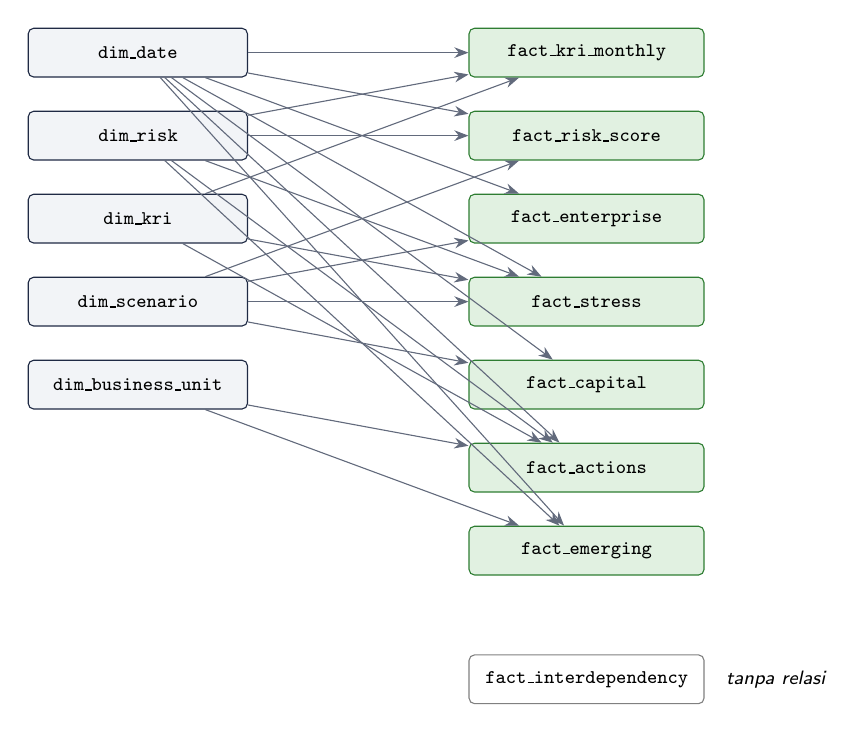
\begin{tikzpicture}[node distance=0.42cm and 0.9cm,
 dim/.style={draw=navy,fill=softgrey,rounded corners=2pt,font=\scriptsize\ttfamily,minimum height=0.62cm,text width=2.55cm,align=center},
 fct/.style={draw=ermgreen,fill=tintgreen!55,rounded corners=2pt,font=\scriptsize\ttfamily,minimum height=0.62cm,text width=2.75cm,align=center},
 lin/.style={-{Stealth[length=1.8mm]},navy!70}]
\node[dim] (date) {dim\_date};
\node[dim,below=of date] (risk) {dim\_risk};
\node[dim,below=of risk] (kri) {dim\_kri};
\node[dim,below=of kri] (scn) {dim\_scenario};
\node[dim,below=of scn] (bu) {dim\_business\_unit};
\node[fct,right=2.8cm of date] (f1) {fact\_kri\_monthly};
\node[fct,below=of f1] (f2) {fact\_risk\_score};
\node[fct,below=of f2] (f3) {fact\_enterprise};
\node[fct,below=of f3] (f4) {fact\_stress};
\node[fct,below=of f4] (f5) {fact\_capital};
\node[fct,below=of f5] (f6) {fact\_actions};
\node[fct,below=of f6] (f7) {fact\_emerging};
\foreach \d in {date,risk,kri} {\draw[lin] (\d) -- (f1);}
\foreach \d in {date,risk,scn} {\draw[lin] (\d) -- (f2);}
\foreach \d in {date,scn} {\draw[lin] (\d) -- (f3);}
\foreach \d in {date,risk,kri,scn} {\draw[lin] (\d) -- (f4);}
\foreach \d in {date,scn} {\draw[lin] (\d) -- (f5);}
\foreach \d in {date,risk,kri,bu} {\draw[lin] (\d) -- (f6);}
\foreach \d in {date,risk,bu} {\draw[lin] (\d) -- (f7);}
\node[fct,below=1.0cm of f7,draw=gray,fill=white] (f8) {fact\_interdependency};
\node[font=\scriptsize\itshape,right=0.15cm of f8] {tanpa relasi};
\end{tikzpicture}
\caption{Peta relasi: lima dimensi memfilter tujuh tabel fakta; tabel interdependency berdiri sendiri.}
\end{figure}

\section{Langkah 3 --- Memasang measure DAX}

\begin{stepbox}{3.1 Buat tabel penampung measure}
\ui{Home} $\rightarrow$ \ui{Enter data} $\rightarrow$ ketik nama tabel \file{\_Measures} $\rightarrow$ \ui{Load}. Tabel kosong berisi satu kolom \file{Column1} akan muncul; biarkan saja (nanti disembunyikan).
\end{stepbox}

\begin{stepbox}{3.2 Tempel measure satu per satu}
Klik tabel \file{\_Measures} di panel \ui{Data} $\rightarrow$ ribbon \ui{Home} $\rightarrow$ \ui{New measure} $\rightarrow$ hapus teks bawaan $\rightarrow$ tempel satu blok rumus dari \file{dashboard/DAX\_measures.md} $\rightarrow$ tekan Enter. Ulangi untuk setiap measure.
\end{stepbox}

\textbf{Urutan pemasangan penting}, karena measure saling memanggil. Pasang berurutan dari atas:

\begin{center}
\begin{tabularx}{\linewidth}{r>{\ttfamily\small}p{5.0cm}X}
\toprule
\textbf{No} & \textrm{\textbf{Measure}} & \textbf{Dipakai di} \\
\midrule
1 & Selected Scenario & Dasar semua measure lain \\
2 & Selected Date Key & Dasar semua measure lain \\
3 & Risk Final Score & Heatmap, matriks, waterfall \\
4 & Risk Model Score & Heatmap (model vs final) \\
5 & Override Delta & Heatmap \\
6 & Risk Score Color & Pewarnaan bersyarat \\
7 & KRI Value & Halaman appetite \\
8 & KRI Score & Halaman appetite dan trend \\
9 & Emerging Risk Count & Kartu halaman 1 \\
10 & Waterfall Contribution & Halaman stress \\
11 & Enterprise Score & Kartu halaman 1 \\
12 & Enterprise Rating & Kartu halaman 1 \\
13 & Limit Utilization \% & Kartu dan gauge \\
14 & Tolerance Breaches & Kartu \\
15 & Limit Breaches & Kartu \\
16 & KRI Score MoM $\Delta$ & Tabel trend \\
17 & Deteriorating KRI Count & Kartu halaman 3 \\
18 & Stress $\Delta$ vs Baseline & Halaman stress \\
19 & Enterprise Stress $\Delta$ vs Baseline & Halaman stress \\
20 & KPMM Stressed & Halaman stress \\
21 & Overdue Actions & Halaman 6 \\
22 & Open Actions & Halaman 6 \\
\bottomrule
\end{tabularx}
\end{center}

\begin{stepbox}{3.3 Atur format angka measure}
Klik measure di panel \ui{Data}, lalu di \ui{Measure tools} atur:
\begin{itemize}
\item \file{Enterprise Score}, \file{Risk Final Score}, \file{Risk Model Score}, \file{KRI Score}: \ui{Decimal number}, 1 desimal
\item \file{Limit Utilization \%} dan \file{KPMM Stressed}: \ui{Percentage}, 1 desimal (kartu boleh 0 desimal)
\item \file{Tolerance Breaches}, \file{Limit Breaches}, \file{Overdue Actions}, \file{Open Actions}, \file{Deteriorating KRI Count}: \ui{Whole number}
\end{itemize}
\end{stepbox}

\begin{tipbox}[Rapikan panel Data]
Sembunyikan kolom teknis agar tidak membingungkan saat menyusun visual: klik kanan kolom $\rightarrow$ \ui{Hide in report view}. Kandidat: semua kolom \file{*\_key}, \file{\_Measures[Column1]}, \file{dim\_date[month\_index]}, dan \file{dim\_date[period]}.
\end{tipbox}

\section{Langkah 4 --- Pengaturan halaman dan slicer}

\begin{stepbox}{4.1 Buat 6 halaman}
Klik tanda \ui{+} di bawah kanvas enam kali, lalu ganti namanya (klik kanan tab $\rightarrow$ \ui{Rename page}):
\begin{enumerate}
\item Enterprise Overview
\item Risk Appetite
\item Risk Trend \& Early Warning
\item Enterprise Stress
\item Interdependency
\item Management Action
\end{enumerate}
\end{stepbox}

\begin{stepbox}{4.2 Slicer bulan (halaman 1, 2, 3, 6)}
Tambahkan visual \ui{Slicer} $\rightarrow$ isi dengan \file{dim\_date[month\_label]} $\rightarrow$ di \ui{Format} $\rightarrow$ \ui{Slicer settings} $\rightarrow$ \ui{Style} pilih \ui{Dropdown} $\rightarrow$ pilih \textbf{Sep-2026}.

Agar seragam di semua halaman: pilih slicer $\rightarrow$ ribbon \ui{Format} $\rightarrow$ \ui{Sync slicers} $\rightarrow$ centang halaman 1, 2, 3, dan 6 pada kolom \ui{Sync} dan \ui{Visible}.
\end{stepbox}

\begin{stepbox}{4.3 Slicer skenario (halaman 4 saja)}
Tambahkan \ui{Slicer} berisi \file{dim\_scenario[scenario]}, style \ui{Tile}, lalu pada \ui{Filters on this visual} $\rightarrow$ \ui{scenario} $\rightarrow$ \ui{Basic filtering} $\rightarrow$ hilangkan centang \textbf{Actual}. Pilih \textbf{Severe} sebagai nilai awal.
\end{stepbox}

\begin{warnbox}[Mengapa slicer skenario penting]
Pada September 2026 ada dua baris di \file{fact\_enterprise}: skenario \texttt{Actual} dan \texttt{Baseline} (angkanya sama). Measure sudah dirancang memakai \texttt{Actual} bila slicer skenario tidak dipilih, sehingga kartu halaman 1 tetap benar. Namun jika Anda membuat visual yang langsung memakai kolom (bukan measure), pastikan skenario difilter agar angka tidak terhitung dua kali.
\end{warnbox}

\section{Langkah 5 --- Menyusun visual per halaman}

Notasi: \ui{Fields} adalah kolom/measure yang Anda tarik ke kotak di panel \ui{Visualizations}.

\subsection{Halaman 1 --- Enterprise Overview}

\begin{enumerate}
\item \textbf{Lima kartu} (\ui{Card}), berjajar di atas: \file{Enterprise Score}, \file{Enterprise Rating}, \file{Limit Utilization \%}, \file{Tolerance Breaches}, \file{Emerging Risk Count}. Tambahkan satu kartu lagi untuk \file{Limit Breaches} bila ingin lengkap.
\item \textbf{Heatmap risiko} (\ui{Matrix}):
  \begin{itemize}
  \item \ui{Rows}: \file{dim\_risk[risk\_type]}
  \item \ui{Values}: \file{Risk Model Score}, \file{Risk Final Score}, \file{Override Delta}
  \item Filter visual: \file{dim\_risk[risk\_type]} \ui{is not} \texttt{Capital Overlay}
  \item Warna: \ui{Format} $\rightarrow$ \ui{Cell elements} $\rightarrow$ pilih seri \file{Risk Final Score} $\rightarrow$ \ui{Background color} $\rightarrow$ \ui{Conditional formatting} $\rightarrow$ \ui{Format style: Field value} $\rightarrow$ \ui{What field should we base this on?}: \file{Risk Score Color}
  \end{itemize}
\item \textbf{Top 3 driver} (\ui{Clustered bar chart}): \ui{Y-axis} \file{dim\_risk[risk\_type]}, \ui{X-axis} \file{Risk Final Score}; pada \ui{Filters} $\rightarrow$ \file{risk\_type} $\rightarrow$ \ui{Top N} $\rightarrow$ \ui{Top} 3 \ui{by} \file{Risk Final Score}.
\item \textbf{Kotak teks} berisi penjelasan singkat, misalnya bahwa Compliance memakai judgment override sehingga skor final lebih tinggi dari model.
\end{enumerate}

\begin{tipbox}[Verifikasi halaman 1 (Sep-2026, tanpa slicer skenario)]
Enterprise Score \textbf{3{,}0} \textbullet{} Rating \textbf{Moderate} \textbullet{} Limit Utilization \textbf{68\%} \textbullet{} Tolerance Breaches \textbf{9} \textbullet{} Limit Breaches \textbf{0} \textbullet{} Emerging Risk \textbf{3}
\end{tipbox}

\subsection{Halaman 2 --- Risk Appetite}

\begin{enumerate}
\item \textbf{Slicer risiko}: \file{dim\_risk[risk\_type]}, style \ui{Dropdown}, \ui{Single select} aktif.
\item \textbf{Slicer KRI}: \file{dim\_kri[kri\_name]}, style \ui{Dropdown}. Slicer ini otomatis menyusut mengikuti risiko yang dipilih karena keduanya terhubung lewat tabel fakta.
\item \textbf{Grafik garis} (\ui{Line chart}):
  \begin{itemize}
  \item \ui{X-axis}: \file{dim\_date[month\_label]}
  \item \ui{Y-axis}: \file{KRI Value}
  \item Garis batas: \ui{Format} $\rightarrow$ \ui{Reference lines} (atau \ui{Analytics}) $\rightarrow$ tambahkan tiga \ui{Constant line} dengan warna hijau, kuning, dan merah. Isi nilainya dari \file{dim\_kri[risk\_appetite]}, \file{[early\_warning\_trigger]}, dan \file{[risk\_limit]} untuk KRI yang sedang dipilih.
  \end{itemize}
\item \textbf{Tabel detail} (\ui{Table}): \file{dim\_kri[kri\_id]}, \file{[kri\_name]}, \file{[unit]}, \file{KRI Value}, \file{dim\_kri[risk\_appetite]}, \file{[early\_warning\_trigger]}, \file{[risk\_limit]}, \file{KRI Score}, \file{fact\_kri\_monthly[utilization]}.
  Warnai kolom \file{KRI Score}: \ui{Conditional formatting} $\rightarrow$ \ui{Field value} $\rightarrow$ \file{fact\_kri\_monthly[color\_hex]} (set agregasi kolom itu ke \ui{First}).
\item \textbf{Gauge}: \ui{Value} \file{Limit Utilization \%}, \ui{Maximum} 1,5 (150\%), \ui{Target} 1 (100\%).
\end{enumerate}

\subsection{Halaman 3 --- Risk Trend \& Early Warning}

\begin{enumerate}
\item \textbf{Matriks 12 bulan}: \ui{Rows} \file{dim\_risk[risk\_type]}, \ui{Columns} \file{dim\_date[month\_label]}, \ui{Values} \file{fact\_risk\_score[final\_score\_display]} (agregasi \ui{Average}). Filter visual: \file{dim\_scenario[scenario]} \ui{is} \texttt{Actual}. Matikan pengaruh slicer bulan: pilih visual $\rightarrow$ ribbon \ui{Format} $\rightarrow$ \ui{Edit interactions} $\rightarrow$ pada slicer bulan pilih ikon \ui{None}.
\item \textbf{Grafik enterprise}: \ui{Line chart} dengan \ui{X-axis} \file{month\_label} dan \ui{Y-axis} \file{fact\_enterprise[enterprise\_score]} (filter skenario \texttt{Actual}). Jangan campur dengan jumlah breach di satu grafik; buat \ui{Column chart} terpisah untuk \file{fact\_enterprise[tolerance\_breaches]}.
\item \textbf{Tabel KRI memburuk}: \file{dim\_kri[kri\_id]}, \file{[kri\_name]}, \file{KRI Value}, \file{KRI Score}, \file{KRI Score MoM $\Delta$}; filter visual \file{fact\_kri\_monthly[trend\_label]} \ui{is} \texttt{Deteriorating}.
\item \textbf{Tabel early warning}: sama, dengan filter \file{fact\_kri\_monthly[early\_warning\_flag]} \ui{is} \texttt{True}.
\item \textbf{Kartu}: \file{Deteriorating KRI Count}.
\end{enumerate}

\begin{tipbox}[Verifikasi halaman 3 (Sep-2026)]
KRI \emph{Deteriorating}: \textbf{18} \textbullet{} KRI \emph{early warning}: \textbf{6} (CP04, LG04, LQ01, LQ05, OR02, RR01)
\end{tipbox}

\subsection{Halaman 4 --- Enterprise Stress}

\begin{enumerate}
\item \textbf{Matriks skenario}: \ui{Rows} \file{dim\_risk[risk\_type]}, \ui{Columns} \file{dim\_scenario[scenario]}, \ui{Values} \file{Risk Final Score}. Warnai dengan \file{Risk Score Color}.
\item \textbf{Tabel ringkasan enterprise}: \ui{Columns} \file{dim\_scenario[scenario]}; \ui{Values} \file{Enterprise Score}, \file{Enterprise Rating}, \file{Limit Utilization \%}, \file{Tolerance Breaches}, \file{Limit Breaches}.
\item \textbf{Waterfall}: visual \ui{Waterfall chart}, \ui{Category} \file{dim\_risk[risk\_type]}, \ui{Y-axis} \file{Waterfall Contribution}. Atur slicer skenario ke \textbf{Severe}.
\item \textbf{Grafik KPMM}: \ui{Clustered column chart}, \ui{X-axis} \file{dim\_scenario[scenario]}, \ui{Y-axis} \file{KPMM Stressed}; tambahkan \ui{Constant line} pada 16\%, 14\%, 12\%, dan 10,5\% sebagai batas skor CAP01.
\item \textbf{Komposisi kerugian}: \ui{Stacked column chart}, \ui{X-axis} \file{dim\_scenario[scenario]}, \ui{Y-axis} \file{fact\_capital[credit\_loss]}, \file{[investment\_loss]}, \file{[op\_loss]}, \file{[dcr\_cost]}.
\item \textbf{Tabel KRI paling terdampak}: \file{dim\_kri[kri\_id]}, \file{[kri\_name]}, \file{fact\_stress[base\_value]}, \file{[stressed\_value]}, \file{[base\_score]}, \file{[stressed\_score]}, \file{[score\_delta]}; urutkan menurun berdasarkan \file{score\_delta}.
\end{enumerate}

\begin{tipbox}[Verifikasi halaman 4]
Skenario \textbf{Severe}: Enterprise \textbf{4{,}0} (Moderate to High) \textbullet{} Limit Utilization \textbf{93\%} \textbullet{} Breach \textbf{21 / 14} \textbullet{} KPMM \textbf{13{,}1\%}. Skenario \textbf{Adverse}: Enterprise \textbf{3{,}4}, KPMM \textbf{15{,}8\%}.
\end{tipbox}

\subsection{Halaman 5 --- Interdependency}

Power BI standar tidak punya visual jaringan. Dua pilihan:

\begin{enumerate}
\item \textbf{Tanpa custom visual (disarankan):} buat \ui{Table} dari \file{fact\_interdependency}: \file{source}, \file{target}, \file{channel}, \file{strength}, \file{evidence}; urutkan \file{strength} menurun. Lengkapi dengan gambar diagram dari laporan PDF halaman 7 (\ui{Insert} $\rightarrow$ \ui{Image}).
\item \textbf{Dengan custom visual:} \ui{Insert} $\rightarrow$ \ui{More visuals} $\rightarrow$ \ui{AppSource} $\rightarrow$ cari \emph{Network Navigator} atau \emph{Sankey}. Isi \ui{Source} = \file{source}, \ui{Target} = \file{target}, \ui{Weight} = \file{strength}.
\end{enumerate}

Tambahkan kotak teks: kenaikan suku bunga acuan adalah pemicu utama, mengalir ke Market, Rate of Return, dan Liquidity.

\subsection{Halaman 6 --- Management Action}

\begin{enumerate}
\item \textbf{Kartu}: \file{Open Actions} dan \file{Overdue Actions}.
\item \textbf{Tabel tracker}: \file{fact\_actions[action\_id]}, \file{dim\_date[month\_label]}, \file{dim\_risk[risk\_type]}, \file{dim\_kri[kri\_id]}, \file{fact\_actions[finding]}, \file{[severity]}, \file{[recommended\_action]}, \file{dim\_business\_unit[business\_unit]}, \file{fact\_actions[due\_date]}, \file{[status]}. Beri warna latar kolom \file{status}: \ui{Conditional formatting} $\rightarrow$ \ui{Rules} (Overdue merah, Open kuning, Closed hijau).
\item \textbf{Donut}: \ui{Legend} \file{fact\_actions[status]}, \ui{Values} jumlah \file{action\_id} (\ui{Count}).
\item \textbf{Tabel emerging risk}: \file{fact\_emerging[er\_id]}, \file{[risk\_name]}, \file{[driver]}, \file{[likelihood]}, \file{[impact]}, \file{[velocity]}, \file{[priority\_score]}, \file{[status]}, \file{[early\_signal]}.
\item \textbf{Scatter}: \ui{X-axis} \file{likelihood}, \ui{Y-axis} \file{impact}, \ui{Size} \file{velocity}, \ui{Legend} \file{status}, \ui{Values} \file{er\_id}.
\end{enumerate}

\begin{warnbox}[Tabel tindakan dan slicer bulan]
Tindakan dibuat pada bulan kejadiannya (Mei s.d. Sep 2026). Jika slicer bulan diarahkan ke Sep-2026, tabel hanya menampilkan 2 tindakan. Agar seluruh 10 tindakan terlihat, matikan interaksi slicer bulan terhadap visual tracker: pilih visual $\rightarrow$ \ui{Format} $\rightarrow$ \ui{Edit interactions} $\rightarrow$ ikon \ui{None} pada slicer bulan.
\end{warnbox}

\begin{tipbox}[Verifikasi halaman 6 (tanpa filter bulan)]
Open \textbf{5} \textbullet{} Overdue \textbf{4} \textbullet{} Closed \textbf{1} \textbullet{} total \textbf{10} tindakan.
\end{tipbox}

\section{Langkah 6 --- Tema warna dan finishing}

\begin{stepbox}{6.1 Warna}
Gunakan tiga warna status secara konsisten: hijau \texttt{\#2E7D32}, kuning \texttt{\#F9A825}, merah \texttt{\#C62828}. Judul dan header memakai navy \texttt{\#1F2A44}. Anda bisa mengaturnya sekali lewat \ui{View} $\rightarrow$ \ui{Themes} $\rightarrow$ \ui{Customize current theme}.
\end{stepbox}

\begin{stepbox}{6.2 Elemen wajib di setiap halaman}
\begin{itemize}
\item Judul halaman (font 20 pt, navy).
\item Kotak teks kecil di bawah: \emph{Fictional bank \textbullet{} synthetic data \textbullet{} project-specific assumptions}.
\item Tanggal posisi data: 30 September 2026.
\end{itemize}
\end{stepbox}

\begin{stepbox}{6.3 Simpan dan bagikan}
\ui{File} $\rightarrow$ \ui{Save as} $\rightarrow$ simpan sebagai \file{dashboard/ERM\_Dashboard.pbix}. Untuk portofolio, ekspor juga tampilannya: \ui{File} $\rightarrow$ \ui{Export} $\rightarrow$ \ui{Export to PDF}.
\end{stepbox}

\section{Pemecahan masalah relasi dan visual}

\begin{longtable}{>{\raggedright\arraybackslash}p{5.9cm}>{\raggedright\arraybackslash}p{8.9cm}}
\toprule
\textbf{Gejala / pesan} & \textbf{Penyebab dan solusi} \\
\midrule
\endhead
\emph{``You can't create a direct active relationship... an active chain already exists''} & Anda mencoba menghubungkan \file{dim\_kri} ke \file{dim\_risk} (atau ke \file{dim\_business\_unit}). Jangan buat relasi itu; tabel fakta sudah punya \file{risk\_key}. \\
\emph{``Both columns contain duplicate values''} & Salah memilih sisi: kolom dim harus unik. Pastikan kolom kunci dim yang dipilih benar (\file{date\_key}, \file{risk\_key}, \file{kri\_key}, \file{scenario\_key}, \file{bu\_key}), bukan kolom lain. \\
Relasi terbentuk tetapi garisnya putus-putus & Relasi menjadi \emph{inactive} karena ada jalur ganda. Hapus relasi yang tidak perlu, biasanya relasi antar-dim. \\
Kolom kunci tidak bisa dipilih & Tipe data berbeda. Samakan menjadi \ui{Whole number} di kedua tabel (Langkah \ref{sec:tipe}). \\
Semua baris visual menampilkan angka yang sama & Relasi ke tabel fakta itu belum ada atau tidak aktif. Periksa di \ui{Model view}. \\
Muncul baris kosong (\emph{blank}) di visual & Ada kunci di fakta yang tidak ada di dim, atau kolom kunci kosong (misalnya \file{source\_risk\_key} pada tabel interdependency). Tambahkan filter visual \ui{is not blank}. \\
Angka kartu halaman 1 dua kali lipat & Visual memakai kolom mentah tanpa filter skenario, sehingga baris \texttt{Actual} dan \texttt{Baseline} dijumlahkan. Gunakan measure, atau tambahkan filter \file{dim\_scenario[scenario]} = \texttt{Actual}. \\
Skor tampil seperti 265 atau 3.0 menjadi 30 & Locale saat impor. Ubah langkah \ui{Changed Type} menjadi \ui{Using Locale: English (United States)}. \\
Bulan tersusun alfabetis (Apr, Ags, Des\ldots) & \file{month\_label} belum diurutkan. Gunakan \ui{Sort by column} $\rightarrow$ \file{month\_index}. \\
\ui{Mark as date table} gagal & Wajar: \file{dim\_date} berisi 12 baris bulanan. Lewati fitur ini; model tidak memerlukannya. \\
Measure error \emph{``cannot find name''} & Measure yang dirujuk belum dibuat. Pasang sesuai urutan di Langkah 3. \\
Tabel tindakan kosong saat slicer Sep-2026 & Tindakan lain dibuat pada Mei--Agustus. Matikan interaksi slicer bulan untuk visual tersebut. \\
\bottomrule
\end{longtable}

\section{Checklist akhir}

\begin{itemize}
\item[$\square$] 13 tabel terimpor, tipe kunci \ui{Whole number}, kolom tanggal \ui{Date}.
\item[$\square$] 21 relasi aktif, arah tunggal, dim $\rightarrow$ fact.
\item[$\square$] Tidak ada relasi antar-dim; \file{fact\_interdependency} berdiri sendiri.
\item[$\square$] 22 measure terpasang dan formatnya benar.
\item[$\square$] 6 halaman tersusun, slicer bulan tersinkron, slicer skenario hanya di halaman 4.
\item[$\square$] Angka verifikasi cocok: Enterprise 3{,}0, RAU 68\%, breach 9/0, KPMM severe 13{,}1\%, overdue actions 4.
\item[$\square$] Warna konsisten dan disclaimer ada di setiap halaman.
\end{itemize}

\vspace{0.6em}
\begin{tcolorbox}[colback=softgrey,colframe=navy,boxrule=0.6pt,arc=2pt,title=Disclaimer,fonttitle=\bfseries]
\small This project uses a fictional Islamic bank and fully synthetic data. All risk appetite thresholds, scenarios, sensitivities, and scoring rules are project-specific analytical assumptions created for educational and portfolio purposes. They do not represent any actual bank's internal limits, regulatory thresholds, or an official OJK risk profile rating.
\end{tcolorbox}

\end{document}
